% Three-panel causal structures for the introduction, version 2 (flatter, 2026-09-23 at the author's request):
% (a) the proxy W as one variable, with a callout for its split into (W_j, W_{-j});
% (b) the held-out block W_j affects Y but not A;
% (c) proximal causal inference with designated proxies.
% Version 1 is 2026-09-23-proximal-balancing-structures.tex.  Changes: the rows are closer (U 1.55, X and the proxies
% 0.72, A and Y -0.15, against 1.65, 0.72, -0.50), the panel labels sit at the top left instead of a row below, and the
% callout sits lower; the panels are spread to about the text width.  X stays in the proxy row, so the crossing edges W -> A and W_{-j} -> Y pass clear below it.
% Same nodes, edges, colours, and fonts.
\documentclass[tikz,border=3pt]{standalone}
\usepackage{amsmath}
\usepackage{sansmath}
\usepackage{xcolor}
\usetikzlibrary{arrows.meta,shapes.callouts}
\definecolor{coltreat}{HTML}{0066CC}
\definecolor{colout}{HTML}{D62828}
\definecolor{collatent}{HTML}{A6A6A6}
\definecolor{filllatent}{HTML}{F2F2F2}
\begin{document}
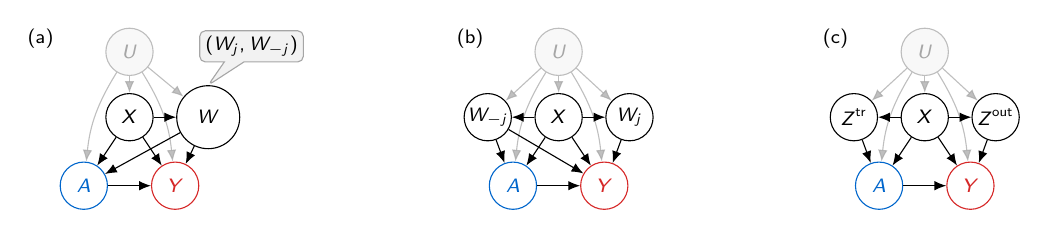
\begin{tikzpicture}[
  x=1cm, y=1cm,
  >={Latex[width=1.2mm,length=1.5mm]},
  font=\sffamily\sansmath\scriptsize,
  varnode/.style={draw,circle,inner sep=0mm,minimum size=6mm,font=\sffamily\sansmath\scriptsize},
  observed/.style={varnode,draw=black,text=black,fill=white},
  latent/.style={varnode,draw=collatent,draw opacity=0.72,text=collatent,fill=filllatent,fill opacity=0.55,text opacity=1},
  treatment/.style={varnode,draw=coltreat,text=coltreat,fill=white},
  outcome/.style={varnode,draw=colout,text=colout,fill=white},
  observed edge/.style={->,draw=black,line width=0.4pt},
  latent edge/.style={->,draw=collatent,opacity=0.72,line width=0.4pt},
  panel label/.style={anchor=north west,inner sep=0pt}
]
% rows: U at 1.55, X and the proxies at 0.72, A and Y at -0.15
% (a) The proxy W as one variable to the right of X; the callout shows its split into blocks.
\begin{scope}[xshift=0cm]
  \node[panel label] at (-1.30,1.85) {(a)};
  \node[latent] (Ua) at (0,1.55) {$U$};
  \node[observed,minimum size=8mm] (Wa) at (1.00,0.72) {$W$};
  \node[observed] (Xa) at (0,0.72) {$X$};
  \node[treatment] (Aa) at (-0.58,-0.15) {$A$};
  \node[outcome] (Ya) at (0.58,-0.15) {$Y$};
  \node[rectangle callout,rounded corners=2pt,draw=collatent,fill=filllatent,text=black,
        inner sep=2pt,callout absolute pointer={(Wa.north)}] at (1.55,1.62) {$(W_j,W_{-j})$};
  \draw[latent edge] (Ua) -- (Wa);
  \draw[latent edge] (Ua) -- (Xa);
  \draw[latent edge] (Ua) to[bend right=13] (Aa);
  \draw[latent edge] (Ua) to[bend left=13] (Ya);
  \draw[observed edge] (Xa) -- (Wa);
  \draw[observed edge] (Xa) -- (Aa);
  \draw[observed edge] (Xa) -- (Ya);
  \draw[observed edge] (Wa) -- (Aa);
  \draw[observed edge] (Wa) -- (Ya);
  \draw[observed edge] (Aa) -- (Ya);
\end{scope}
% (b) Held-out block W_j affects Y but not A; the remaining blocks W_{-j} affect A and Y.
\begin{scope}[xshift=5.45cm]
  \node[panel label] at (-1.30,1.85) {(b)};
  \node[latent] (Ub) at (0,1.55) {$U$};
  \node[observed] (Wmb) at (-0.90,0.72) {$W_{-j}$};
  \node[observed] (Xb) at (0,0.72) {$X$};
  \node[observed] (Wjb) at (0.90,0.72) {$W_j$};
  \node[treatment] (Ab) at (-0.58,-0.15) {$A$};
  \node[outcome] (Yb) at (0.58,-0.15) {$Y$};
  \draw[latent edge] (Ub) -- (Wmb);
  \draw[latent edge] (Ub) -- (Xb);
  \draw[latent edge] (Ub) -- (Wjb);
  \draw[latent edge] (Ub) to[bend right=13] (Ab);
  \draw[latent edge] (Ub) to[bend left=13] (Yb);
  \draw[observed edge] (Xb) -- (Wmb);
  \draw[observed edge] (Xb) -- (Wjb);
  \draw[observed edge] (Xb) -- (Ab);
  \draw[observed edge] (Xb) -- (Yb);
  \draw[observed edge] (Wmb) -- (Ab);
  \draw[observed edge] (Wmb) -- (Yb);
  \draw[observed edge] (Wjb) -- (Yb);
  \draw[observed edge] (Ab) -- (Yb);
\end{scope}
% (c) Proximal causal inference with designated treatment-side and outcome-side proxies.
\begin{scope}[xshift=10.10cm]
  \node[panel label] at (-1.30,1.85) {(c)};
  \node[latent] (Uc) at (0,1.55) {$U$};
  \node[observed] (Ztc) at (-0.90,0.72) {$Z^{\mathrm{tr}}$};
  \node[observed] (Xc) at (0,0.72) {$X$};
  \node[observed] (Zoc) at (0.90,0.72) {$Z^{\mathrm{out}}$};
  \node[treatment] (Ac) at (-0.58,-0.15) {$A$};
  \node[outcome] (Yc) at (0.58,-0.15) {$Y$};
  \draw[latent edge] (Uc) -- (Ztc);
  \draw[latent edge] (Uc) -- (Xc);
  \draw[latent edge] (Uc) -- (Zoc);
  \draw[latent edge] (Uc) to[bend right=13] (Ac);
  \draw[latent edge] (Uc) to[bend left=13] (Yc);
  \draw[observed edge] (Xc) -- (Ztc);
  \draw[observed edge] (Xc) -- (Zoc);
  \draw[observed edge] (Xc) -- (Ac);
  \draw[observed edge] (Xc) -- (Yc);
  \draw[observed edge] (Ztc) -- (Ac);
  \draw[observed edge] (Zoc) -- (Yc);
  \draw[observed edge] (Ac) -- (Yc);
\end{scope}
\end{tikzpicture}
\end{document}
